%%%%%%%%%%%%%%%%%%%%%%%%%%%%%%%%%%%%%%%%%
%
% (c) 2020 by Jennifer Laaser
%
% This work is licensed under the Creative Commons Attribution-NonCommercial-ShareAlike 4.0 International License. To view a copy of this license, visit http://creativecommons.org/licenses/by-nc-sa/4.0/ or send a letter to Creative Commons, PO Box 1866, Mountain View, CA 94042, USA.
%
% The current source for these materials is accessible on Github: https://github.com/jlaaser/pogil-polymers
%
%%%%%%%%%%%%%%%%%%%%%%%%%%%%%%%%%%%%%%%%%

\renewcommand{\figpath}{content/intro/size-and-complexity/figs}
\renewcommand{\labelbase}{size-and-complexity}

\begin{activity}{With Increasing Size Comes Increasing Complexity}

\begin{instructornotes}

	This activity introduces students to key concepts related to the size and molecular weight of polymer molecules, and conformational flexibility.
	
	After completing this activity, students will be able to:
			\begin{enumerate}
				\item Calculate the molecular weight of a polymer, given the number of repeat units and molecular weight of each repeat (and calculate number of repeat units given molecular weight)
				\item Estimate the physical extent of a polymer that is (a) fully extended, (b) fully collapsed, or (c) somewhere inbetween
				\item Estimate the number of conformations available for a single polymer molecule
			\end{enumerate}
			
	\subsection*{Activity summary:}
	\begin{itemize}
		\item \textbf{Activity type:} Learning Cycle
		\item \textbf{Content goals:} Introduction to polymers
		\item \textbf{Process goals:} %https://pogil.org/uploads/attachments/cj54b5yts006cklx4hh758htf-process-skills-official-pogil-list-2015-original.pdf
			written communication, critical thinking, information processing
		\item \textbf{Duration:} 35-40 minutes, including class discussion
		\item \textbf{Instructor preparation required:} none beyond knowledge of relevant content
		\item \textbf{Related textbook chapters:}
			\begin{itemize}
				\item \emph{Polymer Chemistry} (Hiemenz \& Lodge): section 1.2
			\end{itemize}
		%\item \textbf{Facilitation notes:}
		%	\begin{itemize}
		%		\item \dots
		%	\end{itemize}
	\end{itemize}
	
\end{instructornotes}




\begin{model}[Molecular Weight and Degree of Polymerization]
\label{\labelbase:mdl:polyethyleneMW}

	The structure of polyethylene is shown below:

	\vspace{6pt}
	\centerline{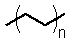
\includegraphics[scale=2]{\figpath/Model1_nrepeats.pdf}}
	\vspace{6pt}
	
	The repeat unit has a chemical formula of \ce{C2H4} and a molecular weight of 28 g/mol.

\end{model}


\begin{ctqs}

	\question Consider a molecule of polyethylene with 100 repeat units.  What would the molecular weight of this molecule be?
			
				\emph{Note: for the purposes of this activity, you may ignore the \ce{CH3} end groups on the chain, and only consider the atoms in the repeat units.}
	
		\begin{solution}[1.5in]
		
			\begin{equation*}
				\left(100\text{ repeat units}\right)\left(\frac{28\text{ g/mol}}{1\text{ repeat unit}}\right) = 2800\text{ g/mol}
			\end{equation*}
		\end{solution}
				
	\question Conversely, consider a molecule of polyethylene with a molecular weight of 700~kg/mol.  Approximately how many repeat units would this chain contain? \label{\labelbase:ctq:700kgPE}
	
		\begin{solution}[1.5in]
		\begin{equation*}
			\left(\frac{700\text{ kg}}{1\text{ mol}}\right)
			\left(\frac{1000\text{ g}}{1\text{ kg}}\right)
			\left(\frac{1\text{ repeat unit}}{28\text{ g/mol}}\right)
			= 25000\text{ repeat units}
		\end{equation*}
		
			As a point of interest, this is in the ballpark for commercial HDPE and LDPE, which typically have degrees of polymerization between 10000 and 100000.
		\end{solution}
	
\end{ctqs}

\begin{infobox}

	Polymer chains are typically synthesized from small molecules called \emph{monomers}.  The number of monomers that make up a polymer chain, $N$, is referred to as the \emph{degree of polymerization}.
	
	For polyethylene, each \ce{C2H4} repeat unit corresponds to exactly one ethylene monomer.

\end{infobox}

\begin{ctqs}
		
	\question What would the molecular weight of a polyethylene molecule made up of $N$ monomers be?
	
		\begin{solution}[1in]
			$28 N$ g/mol
		\end{solution}
		
	\question More generally, suppose a polymer chain is made up of $N$ monomers that each have molecular weight $M_0$.  What would the molecular weight of this polymer be?
	
		\begin{solution}[1in]
			$M_0 N$
		\end{solution}
	
	\question Explain, in 1-2 complete sentences, how you could calculate each of the following:
	
		\begin{enumerate}
			\item The molecular weight of a polymer, if you knew the degree of polymerization and the molecular weight of each monomer:
	
		\begin{solution}[1.75in]
			To obtain the molecular weight of the polymer, you would multiply the degree of polymerization by the molecular weight of the monomer ($M = M_0 N$).
		\end{solution}
			
			\item The degree of polymerization, if you knew the molecular weight of the polymer and the molecular weight of each monomer:
	
		\begin{solution}[1.75in]
			To obtain the degree of polymerization, you would divide the molecular weight of the polymer by the molecular weight of the monomer ($N = \frac{M}{M_0}$).
		\end{solution}
		
		\end{enumerate}
	
\end{ctqs}



\begin{model}[Sizes of Polymer Chains]
	\label{\labelbase:mdl:polyethylenesize}
	
	Carbon-carbon single bonds are typically approximately 1.5~\AA\ long.  Because the bond angle in linear alkanes is approximately 109.5${}^\circ$, every two carbon-carbon bonds contributes approximately 0.25~nm to the length of a polymer chain when it is in its fully extended conformation:
	
	\vspace{6pt}
	\centerline{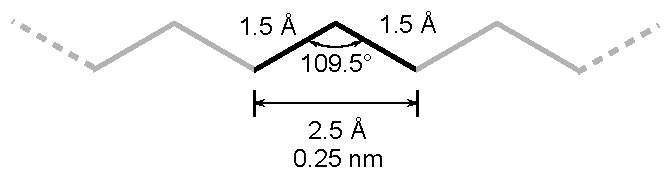
\includegraphics[width=0.7\textwidth]{\figpath/Model2_extendedchain.pdf}}

\end{model}

\begin{ctqs}

	\question How many carbon-carbon bonds does each repeat unit contribute to a polyethylene chain?
	
		\emph{Note: make sure to pay attention not only to the bond in the middle of each repeat unit, but also the bonds that connect different repeat units - how should you count these?}
		
		\begin{solution}[1in]
			2
		\end{solution}
	
	\question How many carbon-carbon bonds would the 700~kg/mol polyethylene molecule in CTQ \ref{\labelbase:ctq:700kgPE} contain?
		
		\begin{solution}[1in]
			$2(25000)\approx 50000$
		\end{solution}
	
	\question Using your answer to the previous question, and the information in Model \ref{\labelbase:mdl:polyethylenesize}, calculate the expected length of this molecule in its fully extended conformation. \label{\labelbase:ctq:extendedPE}
		
		\begin{solution}[1.9in]
			\begin{equation*}
				\left(50000\text{ C-C bonds}\right)\left(\frac{0.25\text{ nm}}{2\text{ C-C bonds}}\right) = 6250\text{ nm} = 6.25~\mu\text{m}
			\end{equation*}
			
			(Note: some students may leave out the factor of 2 in the denominator in this problem, but will likely self-correct quickly during discussion.)
			
			Students may find it interesting to consider that this is comparable to the dimensions of a red blood cell - it is very large for a single molecule!
		\end{solution}
	\question Suppose that instead of stretching the chain out, we collapsed it into a sphere with the same density as bulk polyethylene (approximately 0.95~g/cm\textsuperscript{3}).  What would the radius of this sphere be? \label{\labelbase:ctq:collapsedPE}
	
		\emph{Hint: you'll need to find the mass of a single chain, and then use the density to calculate how much volume it takes up.  You'll probably find it useful to remember that Avogadro's number is approximately 6.022$\times 10^{23}$, and the volume of a sphere of radius $R$ is $\frac{4}{3}\pi R^3$.}
		
		\begin{solution}[3.85in]
			First, let's calculate the volume of a single polymer chain:
			\begin{equation*}
				\left(\frac{700\text{ kg}}{1\text{ mol}}\right)
				\left(\frac{1\text{ mol}}{6.022\times10^{23}\text{ molecules}}\right)
				\left(\frac{1\text{ cm}^3}{0.95\text{ g}}\right)
				\left(\frac{1000\text{ g}}{1\text{ kg}}\right)
				= 1.22 \times 10^{-18}\text{ cm}^3
			\end{equation*}
			Rearranging the equation for the volume of a sphere to solve for radius, we obtain
			\begin{equation*}
				R=\sqrt[3]{\frac{3 V}{4\pi}} = \sqrt[3]{\frac{3 \left(1.22 \times 10^{-18}\text{ cm}^3\right)}{4\pi}} = 6.6 \times 10^{-7}\text{ cm} = 6.6\text{ nm}
			\end{equation*}
			This is three orders of magnitude smaller than the fully extended chain discussed in the previous problem!
		\end{solution}
		
	\question In practice, a 700~g/mol polyethylene chain will typically have a spatial extent on the order of 40~nm.  
	
		\begin{enumerate}
			\item Is this closer to your estimate from CTQ \ref{\labelbase:ctq:extendedPE} or CTQ \ref{\labelbase:ctq:collapsedPE}?
			
				\begin{solution}[0.5in]\instructordisplay{
					This value is closer to the radius of the collapsed chain calculated in CTQ \ref{\labelbase:ctq:collapsedPE}.
				}\end{solution}
			
			\item What does your answer tell you about whether polymer chains are typically more extended or more collapsed?  Explain your answer in 1-2 complete sentences.
			
				\begin{solution}[1.75in]
					This result suggests that polymer chains are typically more collapsed than extended.  However, because the spatial extent is still almost an order of magnitude larger than expected for the fully collapsed globule, the chain can't be fully collapsed, and is likely more of a loose coil.
				\end{solution}
			
		\end{enumerate}
		
\end{ctqs}



\begin{model}[Conformations of Polymer Chains]
	\label{\labelbase:mdl:conformations}

	As seen in Model \ref{\labelbase:mdl:polyethylenesize}, polymer chains may have many different conformations.  In fact, each carbon-carbon bond in polyethylene can take one of three different conformations:
	
	\vspace{6pt}
	\centerline{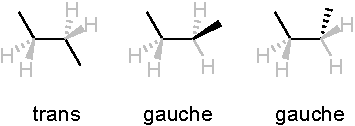
\includegraphics[width=0.5\textwidth]{\figpath/Model3_conformations.pdf}}
	
	As a result, the total number of conformations of a molecule with $n$ carbon-carbon bonds is $3^n$.

\end{model}

\begin{ctqs}

	\question How many possible conformations does the 700~kg/mol molecule of polyethylene considered earlier in this activity have?
	
		\begin{solution}[1in]
			\begin{equation*}
				3^{\text{\# of C-C bonds}} = 3^{50000} \approx 10^{23850}
			\end{equation*}
		\end{solution}
	
	\question 1~kg of 700~kg/mol polyethylene would contain approximately $9\times 10^{20}$ molecules.  Using this information, critique or defend the following statement in 2-3 complete sentences:
	
		\emph{``On average, a polymer sample will contain many molecules in each conformation.''}
	
		\begin{solution}[2.5in]
		
			This statement is false.  The number of possible conformations is much, much larger than the number of molecules in the sample, by thousands of orders of magnitude.  Thus the polymer chains the sample almost certainly all have different conformations, and it is very unlikely that any two are the same.
		\end{solution}
		
\end{ctqs}


\begin{exercises}

	\exercise In Model \ref{\labelbase:mdl:polyethyleneMW} (and the rest of this activity), we ignored the molecular weight of the end groups.  To determine whether or not this was a reasonable approximation, do the following:
	
		\begin{enumerate}
			
			\item Derive a formula for the molecular weight of a polyethylene molecule containing only $N$ \ce{C2H4} repeat units (i.e. without counting the end groups).
			
				\begin{solution}\instructordisplay{
					Each \ce{C2H4} repeat has a molecular weight of 28 g/mol, so the molecular weight is 28*$N$ g/mol.
				}\end{solution}
			
			\item Derive a formula for the molecular weight of a polyethylene molecule containing $N$ \ce{C2H4} repeat units and two \ce{CH3} end groups.
			
				\begin{solution}\instructordisplay{
					Each \ce{C2H4} repeat has a molecular weight of 28 g/mol, while each \ce{CH3} end group has a molecular weight of 15 g/mol, so the correct formula is (28*N + 2*15) g/mol.
				}\end{solution}
			
			\item Calculate the molecular weight obtained from each formula for $N=10$, $N=20$, $N=50$, $N=100$, $N=200$, and $N=500$. For each value of $N$, what is the percent error in the estimate obtained when you ignore the end groups, and above what degree of polymerization would you judge this error to be negligible?
			
				\begin{solution}\instructordisplay{
					The calculated values are:
					
					\begin{center}
						\begin{tabular}{cccc}
						\hline
N   & MW with end groups (g/mol) & MW without end groups (g/mol) & \% error \\\hline
10  & 310                        & 280                           & -9.7     \\
20  & 590                        & 560                           & -5.1     \\
50  & 1430                       & 1400                          & -2.1     \\
100 & 2830                       & 2800                          & -1.1     \\
200 & 5630                       & 5600                          & -0.5     \\
500 & 14030                      & 1400                          & -0.2  
\\\hline  
\end{tabular}
					\end{center}
					
					The N value above which students judge the correction to be negligible depends on how much error they are willing to accept, but using 1\% as a good rule of thumb, the correction is negligible when the chains have 100 or more repeat units.

Note: all of the \% errors should be negative - the molecular weight when end groups are ignored is always lower than the correct molecular weight.

				}\end{solution}
			
		\end{enumerate}
		
	\exercise Summarize, in your own words, the key ways in which polymers differ from small molecules.
	
		\begin{solution}\instructordisplay{
			The key ways in which polymers differ from small molecules include:

\begin{enumerate}
	\item Their physical size: polymers have physical sizes ranging from a few nanometers, in their fully collapsed states, to several microns, in their fully extended conformations.  This is much larger than - and a much larger range than - small molecules.
	\item Their molecular weights: polymers have molecular weights in the thousands to millions of grams per mole, while small molecules rarely have molecular weights greater than a few hundred grams per mole.  The large molecular weights mean that intermolecular interactions between polymers are typically strong, which affects their physical properties (e.g. state of matter, solubility, viscosity, etc. - see previous Activity).
	\item Their number of accessible conformations: polymer molecules typically have so many conformations that it is impossible to enumerate them or to have more than one of each conformation in a sample.  Small molecules, on the other hand, typically only have a handful of conformations that can be enumerated exactly.
\end{enumerate}

Although not addressed in this Activity, once students are introduced to the concepts of dispersity, composition, tacticity, and topology they should additionally recognize that polymers also differ from small molecules in their heterogeneity: polymer samples can contain molecules with different molecular weights, different compositions, different stereochemistries, and potentially different connectivity.  This heterogeneity means that we always have to think about polymers in terms of averages over large numbers of molecules rather than as a single well-defined structure.

		}\end{solution}
	
\end{exercises}


%\begin{problems}

%	\problem First exercise
%	\problem Second exercise
	
%\end{problems}


	
\end{activity}